\chapter{Specifikacija programske potpore}
		
	\section{Funkcionalni zahtjevi}
			
			\noindent \textbf{Dionici:}
			
			\begin{packed_enum}
				
				\item Administrator
				\item Voditelj			
				\item Autor
				\item Posjetitelj
				\item Razvojni tim
				
			\end{packed_enum}
			
			\noindent \textbf{Aktori i njihovi funkcionalni zahtjevi:}
			
			
			\begin{packed_enum}
				\item  \underbar{Neregistrirani korisnik (inicijator) može:}
				
				\begin{packed_enum}
					
					\item stvoriti novi račun registracijom za koju su mu potrebni ime i prezime, e-mail, korisničko ime, lozinka i broj mobitela
					\item pregledati kalendar događaja, odnosno može vidjeti:
					\begin{packed_enum}
						
						\item  vrijeme konferencije
						\item  mjesto konferencije
				
					\end{packed_enum}
					
				\end{packed_enum}

				\item  \underbar{Posjetitelj (inicijator) može:}
				
				\begin{packed_enum}
					
					\item upravlajti svojim osobnim podacima
					\item pokrenuti direktno video praćenje događaja u glavnoj dvorani
					\item glasati za točno jedan poster
					\item spremati fotografije lokalno na svoj uređaj
					\item 

				\end{packed_enum}

				\item  \underbar{Autor (inicijator) može:}
				
				\begin{packed_enum}
					
					\item poslati odgovarajuće materijale voditelju putem e-maila
					\item dobiti inforamcije o svom rangu na konferenciji putem e-maila
					
				\end{packed_enum}

				\item  \underbar{Voditelj (inicijator) može:}
				
				\begin{packed_enum}
					
					\item prijaviti autora
					\item prijaviti stručni rad
					\item prijaviti poster
					\item postavljati fotografije tijekom konferencije
					
				\end{packed_enum}

				\item  \underbar{Administrator (inicijator) može:}
				
				\begin{packed_enum}
					
					\item vidjeti sve podatke svakog registriranog korisnika
					\item obrisati korisnički račun ili mu promijeniti status
					\item dodati i/ili izbrisati konferenciju s kalendara
					\item dodati i/ili izbrisati poster
					
				\end{packed_enum}

			
				\item  \underbar{Baza podataka (sudionik):}
				
				\begin{packed_enum}
					
					\item sadrži podatke o svim korisnicima i njihovom statusu
					\item sadrži podatke o svim održanim ili budućim konferencijama
					\item sadrži podatke o svakom posteru, autoru, broju glasova i krajnjem rangu
					
				\end{packed_enum}
			\end{packed_enum}
			
			\eject 
			
			
				
			\subsection{Obrasci uporabe}
				
				\subsubsection{Opis obrazaca uporabe}
					
					\noindent \underbar{\textbf{UC1 -Registracija}}
					\begin{packed_item}
	
						\item \textbf{Glavni sudionik: }Autor, posjetitelj
						\item  \textbf{Cilj:} stvoriti korisnički račun za prijavu u sustav
						\item  \textbf{Sudionici:} Baza podataka
						\item  \textbf{Preduvjet:} -
						\item  \textbf{Opis osnovnog tijeka:}
						
						\item[] \begin{packed_enum}
	
							\item Korisnik odabere opciju za registraciju
							\item Unosi potrebne korisničke podatke
							\item Obavještava ga se o uspješno registracijii
						\end{packed_enum}
						
						\item  \textbf{Opis mogućih odstupanja:}
						
						\item[] \begin{packed_item}
	
							\item Unos postojećeg ili nezadovoljavajuće e-maila

							\item[] \begin{packed_enum}
								
								\item Obavještavanje korisnika o neuspjeloj registraciji
								\item Vraćanje korisnika na početak tj. ponovnu registracij
								\item Korisnik mijenja podatke ili odustaje od registracije
								
							\end{packed_enum}
							
						\end{packed_item}
					\end{packed_item}

					\noindent \underbar{\textbf{UC2 -Pregled konferencija}}
					\begin{packed_item}
	
						\item \textbf{Glavni sudionik: }Autor, posjetitelj
						\item  \textbf{Cilj:} Pregled konferencija
						\item  \textbf{Sudionici:} Baza podataka
						\item  \textbf{Preduvjet:} -
						\item  \textbf{Opis osnovnog tijeka:}
						
						\item[] \begin{packed_enum}
	
							\item Sve dostupne konferencije su prikazane prilikom otvaranja aplikacije
							\item Korisnik odabire konferenciju koji hoće
							\item Prije nego mu se dopusti pristup konferenciji korisnik treba biti registriran
						\end{packed_enum}
						
					\end{packed_item}

					\noindent \underbar{\textbf{UC3 -Pregled radova}}
					\begin{packed_item}
	
						\item \textbf{Glavni sudionik: }Autor, posjetitelj
						\item  \textbf{Cilj:} Pregled konferencija
						\item  \textbf{Sudionici:} Baza podataka
						\item  \textbf{Preduvjet:} Registracija u sustav, prijavljen u konferenciju
						\item  \textbf{Opis osnovnog tijeka:}
						
						\item[] \begin{packed_enum}
	
							\item Ulazak na neku određenu konferenciju
							\item Prikaz svih radova 
						\end{packed_enum}
						
					\end{packed_item}

					\noindent \underbar{\textbf{UC4 -Ocjenjivanje radova}}
					\begin{packed_item}
	
						\item \textbf{Glavni sudionik: }Posjetitelj
						\item  \textbf{Cilj:} Davanje svog glasa jednom od radova
						\item  \textbf{Sudionici:} Baza podataka, posjetitelj
						\item  \textbf{Preduvjet:} Uspješna prijava u konferenciju
						\item  \textbf{Opis osnovnog tijeka:}
						
						\item[] \begin{packed_enum}
	
							\item Odabir rada kojem se odlučuje dati glas 
							\item Davanje glasa odabranom radu
						\end{packed_enum}
						
					\end{packed_item}

					\noindent \underbar{\textbf{UC5 -Prijava u konferenciju}}
					\begin{packed_item}
	
						\item \textbf{Glavni sudionik: }Autor, posjetitelj
						\item  \textbf{Cilj:} Prijava u konferenciju radi pregleda radova
						\item  \textbf{Sudionici:} Baza podataka
						\item  \textbf{Preduvjet:} Registracija korisnik
						\item  \textbf{Opis osnovnog tijeka:}
						
						\item[] \begin{packed_enum}
	
							\item Odabir određene konferencije za koju želite pristup
							\item Upisivanje lozinke za tu konferenciju uz uvjet da ste prijavljeni
							\item Dobivanje pristupa konferenciji
						\end{packed_enum}
						
					\end{packed_item}

					\noindent \underbar{\textbf{UC6-Dodavanje voditelja/otvaranje nove konferencije}}
					\begin{packed_item}
	
						\item \textbf{Glavni sudionik: }Administrator
						\item  \textbf{Cilj:} Otvaranje konferencije
						\item  \textbf{Sudionici:} Baza podataka, Administrator, Voditelj
						\item  \textbf{Preduvjet:} Odobrenje administratora
						\item  \textbf{Opis osnovnog tijeka:}
						
						\item[] \begin{packed_enum}
	
							\item Kontaktiranje administratora radi otvaranja nove konferencije
							\item Otvaranje konferencije od strane administratora te dodjeljivanje voditelja
						\end{packed_enum}
						
					\end{packed_item}

					\noindent \underbar{\textbf{UC7 -Pregled vremenske prognoze}}
					\begin{packed_item}
	
						\item \textbf{Glavni sudionik: }Autor, posjetitelj
						\item  \textbf{Cilj:} Pregled vremenske prognoze za određenu konferenciju
						\item  \textbf{Sudionici:} Baza podataka
						\item  \textbf{Preduvjet:} Registracija korisnika, odabir konferencije
						\item  \textbf{Opis osnovnog tijeka:}
						
						\item[] \begin{packed_enum}
	
							\item Nakon odabrane konferencije na dnu stranice će biti moguće vidjeti vremensku prognozu za lokaciju te konferencije$>$
						\end{packed_enum}
						
					\end{packed_item}

					\noindent \underbar{\textbf{UC8-Dodavanje rada u konferenciju}}
					\begin{packed_item}
	
						\item \textbf{Glavni sudionik: }Autor, voditelj
						\item  \textbf{Cilj:} Dodavanje/prijava rada na nekoj konferenciji
						\item  \textbf{Sudionici:} Baza podataka, Voditelj, Autor
						\item  \textbf{Preduvjet:} -
						\item  \textbf{Opis osnovnog tijeka:}
						
						\item[] \begin{packed_enum}
	
							\item Autor šalje mail s radom voditelju konferencije
							\item Voditelj konferencije dodaje rad u konferenciju kako bi se mogao prikazati
						\end{packed_enum}
						
					\end{packed_item}

					\noindent \underbar{\textbf{UC9-Video praćenje konferencije}}
					\begin{packed_item}
	
						\item \textbf{Glavni sudionik: }Posjetitelj
						\item  \textbf{Cilj:} Praćenje konferencije online
						\item  \textbf{Sudionici:} Baza podataka, posjetitelj
						\item  \textbf{Preduvjet:} Registracija korisnika
						\item  \textbf{Opis osnovnog tijeka:}
						
						\item[] \begin{packed_enum}
	
							\item Korisnik se mora registrirati
							\item Nakon što je korisnik registriran može odabrati online praćenje
						\end{packed_enum}
						
					\end{packed_item}
				
				
					
				\subsubsection{Dijagrami obrazaca uporabe}
					
		\begin{figure}[H]
			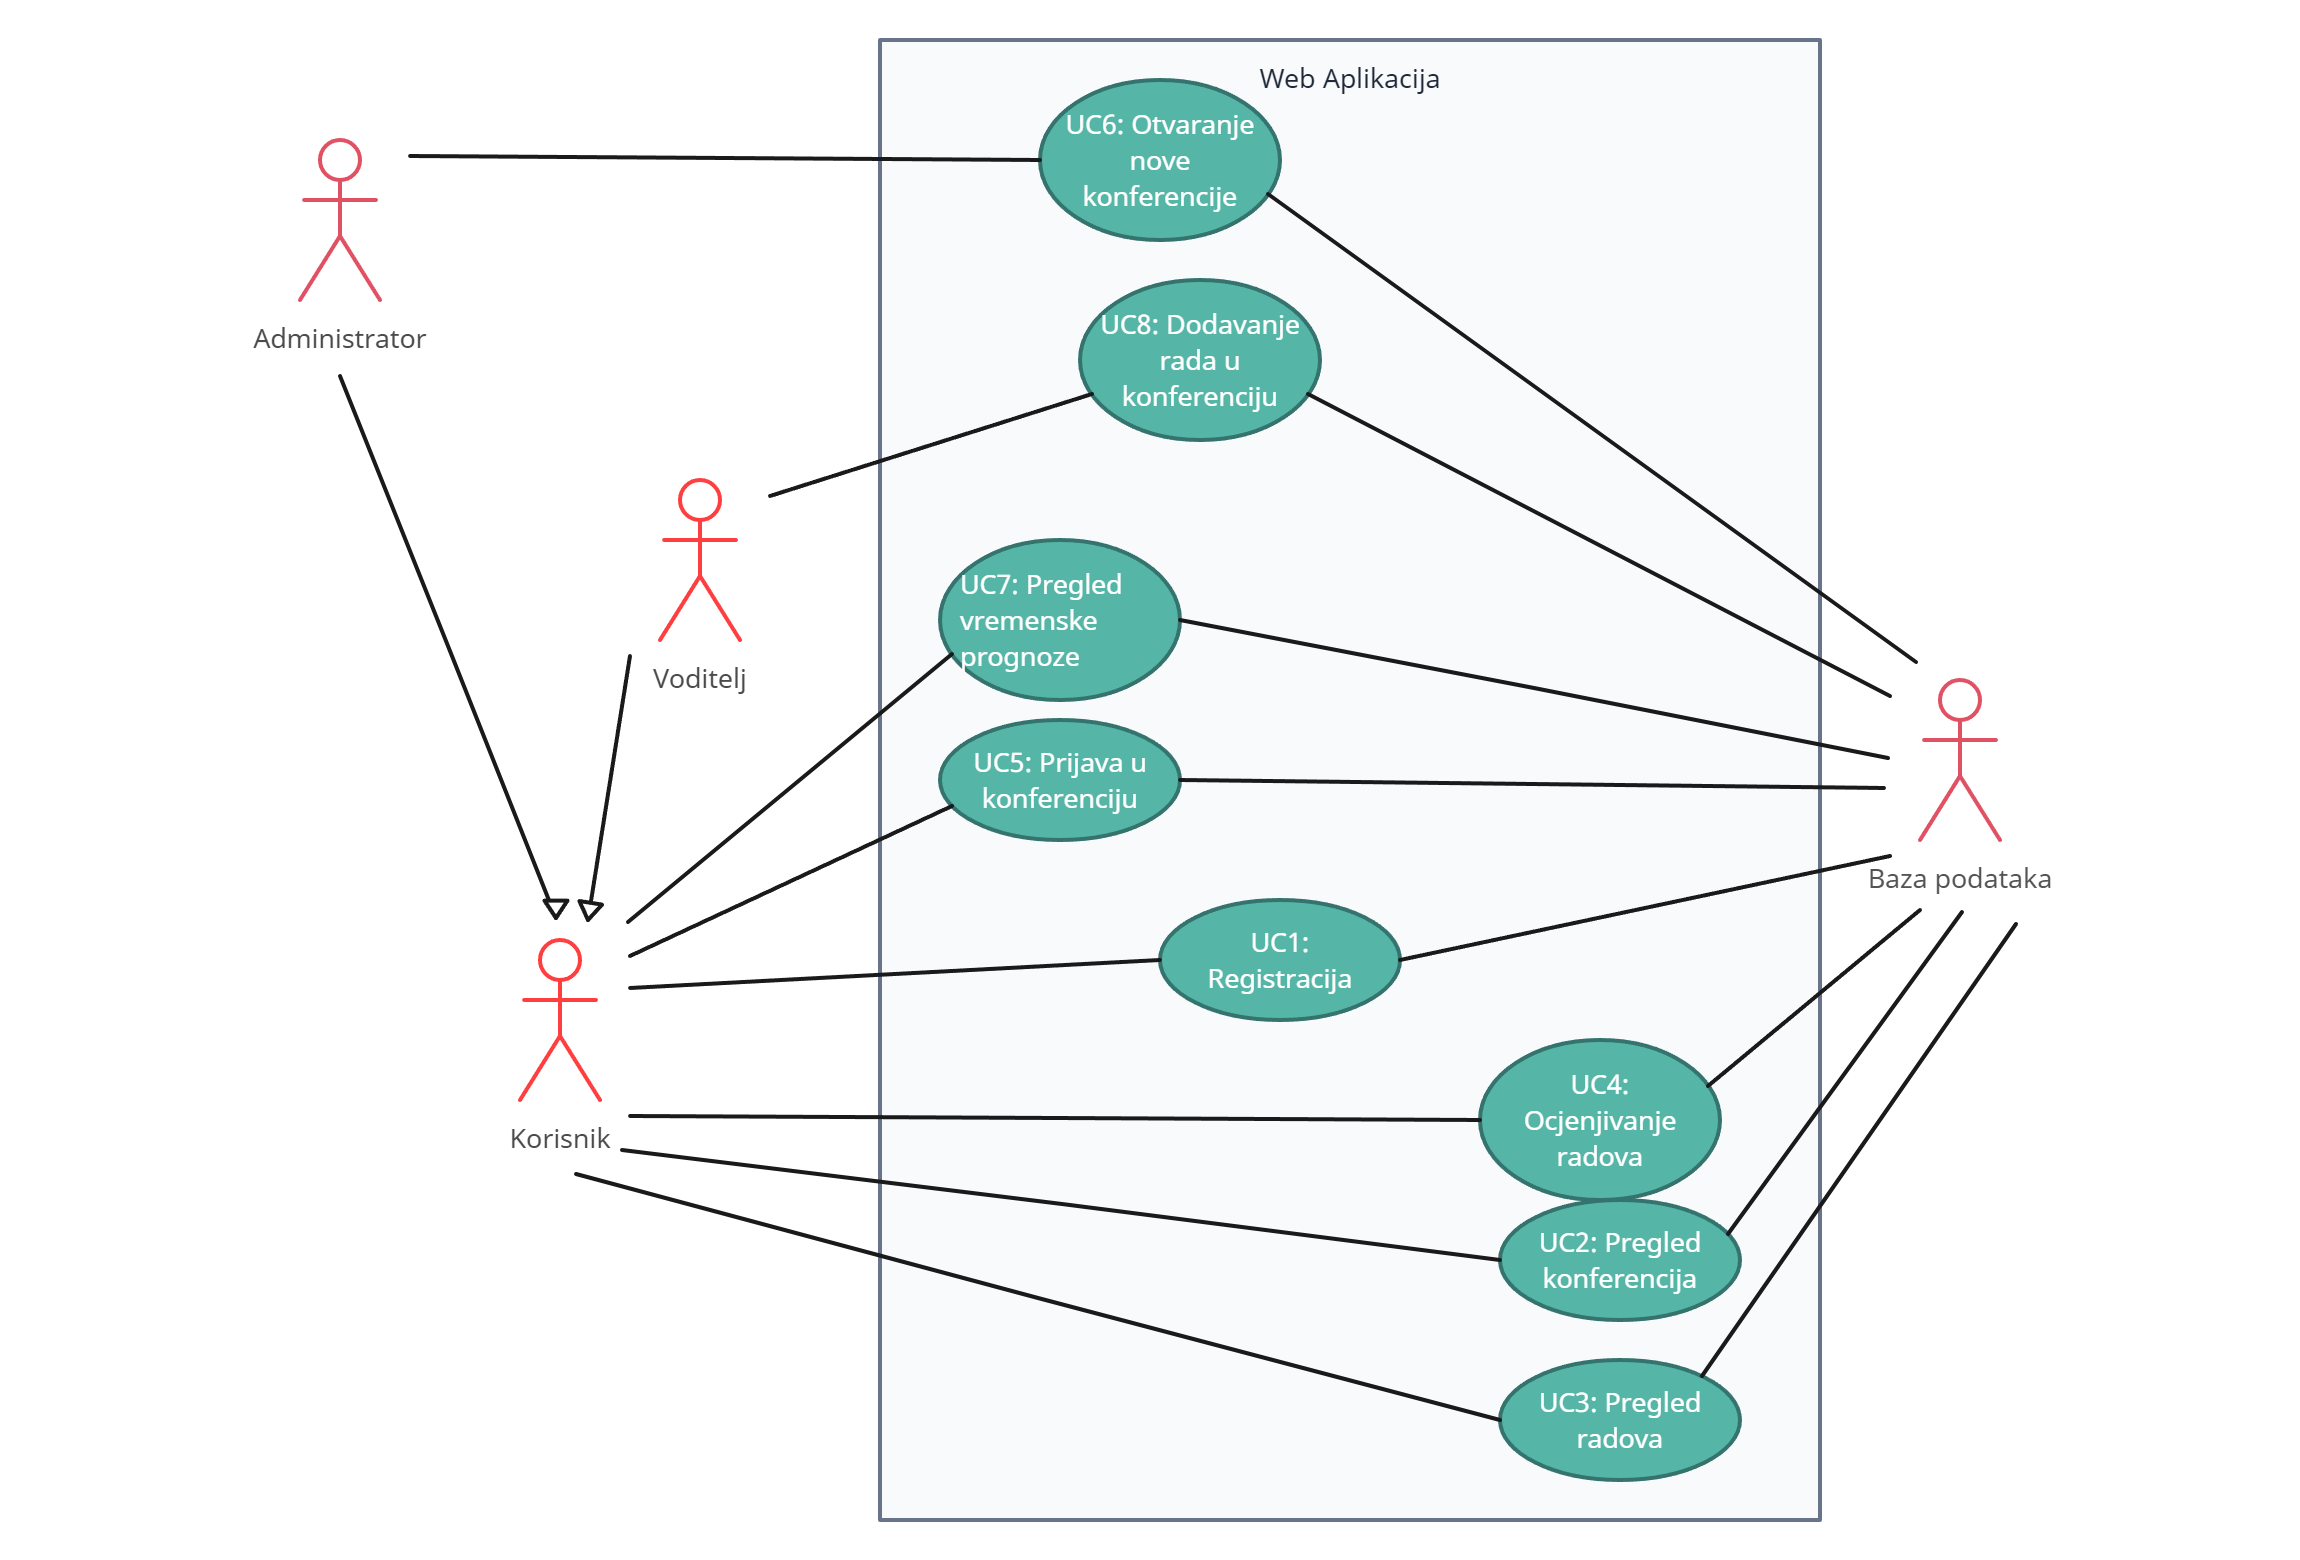
\includegraphics[scale=0.55]{slike/UML1.JPG} 
			\centering
			\caption{Slika 3.1: }
			\label{UML1}
		\end{figure}		
				
			\subsection{Sekvencijski dijagrami}
				
		\begin{figure}[H]
			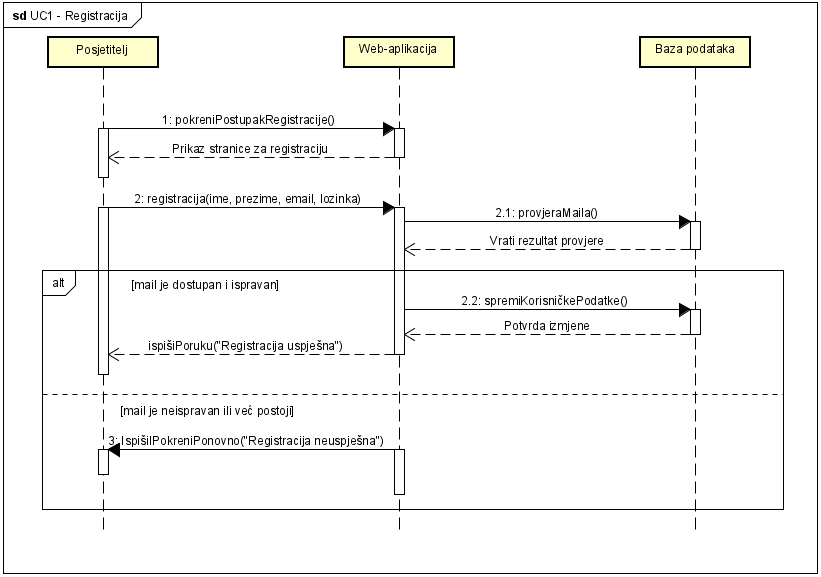
\includegraphics[scale=0.7]{slike/UC1.PNG} 
			\centering
			\caption{Slika 3.2: Sekvencijski dijagram za UC1}
			\label{fig:UC1}
		\end{figure}	

		\begin{figure}[H]
			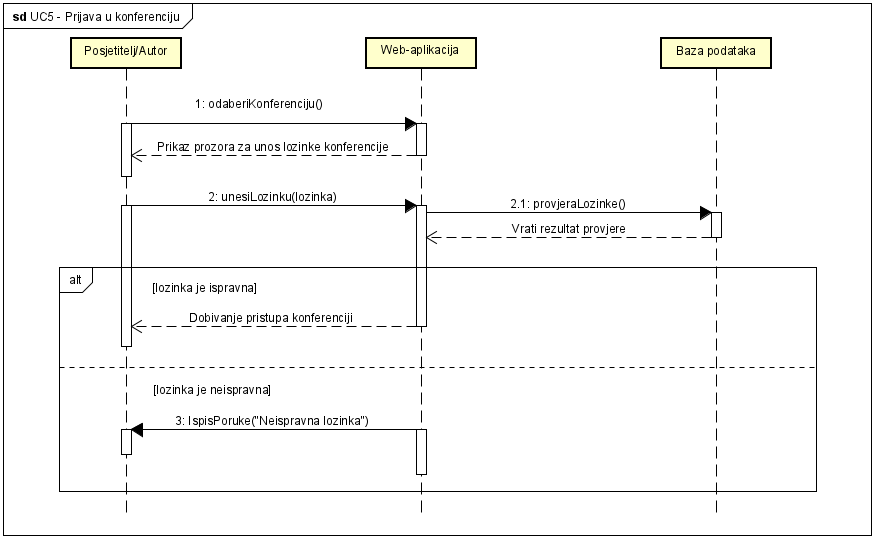
\includegraphics[scale=0.7]{slike/UC5.PNG} 
			\centering
			\caption{Slika 3.3: Sekvencijski dijagram za UC5}
			\label{fig:UC5}
		\end{figure}	
	
		\section{Ostali zahtjevi}
		
			\textbf{\textit{dio 1. revizije}}\\
		 
			 \textit{Nefunkcionalni zahtjevi i zahtjevi domene primjene dopunjuju funkcionalne zahtjeve. Oni opisuju \textbf{kako se sustav treba ponašati} i koja \textbf{ograničenja} treba poštivati (performanse, korisničko iskustvo, pouzdanost, standardi kvalitete, sigurnost...). Primjeri takvih zahtjeva u Vašem projektu mogu biti: podržani jezici korisničkog sučelja, vrijeme odziva, najveći mogući podržani broj korisnika, podržane web/mobilne platforme, razina zaštite (protokoli komunikacije, kriptiranje...)... Svaki takav zahtjev potrebno je navesti u jednoj ili dvije rečenice.}
			 
			 
			 
	